\addchap{How to Use This Book}

\tikzset{
	depnode/.style={
		rounded corners=2pt, draw, line width=0.5pt, inner sep=3pt,
		text width=2.9cm, align=center, font=\scriptsize,
		minimum height=0.55cm
	},
	depia/.style={depnode, fill=black!6,        draw=black!45},
	depib/.style={depnode, fill=RoyalBlue!10,   draw=RoyalBlue!55},
	depii/.style={depnode, fill=purple!10,      draw=purple!55},
	deparrow/.style={->, >=stealth, draw=black!45, line width=0.5pt, shorten >=1pt}
}

\section*{The shape of the book}

The book is in three parts, matching the three years of the Cambridge Mathematical
Tripos, and each part is a year's worth of lectures.

\begin{itemize}
	\item \textbf{Part IA} (eight chapters) is the first year. Everybody takes everything;
	there is no choice at all.
	\item \textbf{Part IB} (fifteen chapters) is the second year, where the syllabus opens
	up and a student picks perhaps ten of the courses on offer. What is collected here
	is what I took.
	\item \textbf{Part II} (twenty-one chapters) is the third year, where the courses
	become genuinely specialised and largely independent of one another.
\end{itemize}

Each of the three parts opens with a short essay about what that year is doing and how
its courses hang together. Those essays are the closest thing this book has to a
narrative, and they are worth reading before the mathematics.

\section*{Every chapter is a course}

This is the single most important thing to know about the book. Each chapter is one
lecture course, written as a standalone document and then dropped in here essentially
untouched. In particular:

\begin{itemize}
	\item \textbf{Chapters do not continue from one another.} Chapter 17 does not pick up
	where Chapter 16 left off; it starts again from its own beginning, with its own
	introduction saying what the course is about.

	\item \textbf{Notation is local.} A macro or a piece of notation established in one
	chapter is dissolved at the end of it. Two chapters may use the same letter for
	completely different things, and two chapters covering overlapping material may
	well use different conventions for it.

	\item \textbf{Numbering is by chapter and section.} A reference to Theorem 4.2.1 means
	the first numbered result in the second section of the fourth chapter. Definitions,
	theorems, lemmas and examples share a single counter within each section, so the
	numbers run in reading order.

	\item \textbf{Occasional references point outwards.} Because these were written as
	separate documents, you will now and then find a phrase like ``see my Numbers and
	Sets notes''. That means the corresponding chapter of this book.
\end{itemize}

The upside of all this is that you can open the book anywhere. The downside is that
reading it front to back is not obviously the right thing to do, which brings us to the
next section.

\section*{Reading order, and the dependency graphs}

Only Part IA is really meant to be read from a standing start. After that the courses
fan out, and by Part II several of them share no content at all -- the reader of
Statistical Physics and the reader of Logic and Set Theory can happily ignore each
other.

My honest advice is not to read this book linearly. Pick a chapter you want, look up
what it stands on, and read backwards until you hit something you already know. The
diagrams below are there to make that possible. They show the main lines of dependency
running through the three years: an arrow from $A$ to $B$ means that $B$ genuinely
leans on $A$, not merely that the two are thematically related. Position from left to
right indicates the direction of that flow, and the colour of a box tells you which
part the course belongs to.

\begin{center}

\begin{tikzpicture}
	\node[depia] at (0,0) {Part IA};
	\node[depib] at (3.4,0) {Part IB};
	\node[depii] at (6.8,0) {Part II};
\end{tikzpicture}
\end{center}

The graphs are deliberately incomplete. Every course assumes the whole of Part IA in
the background, and drawing that in would have turned each picture into a scribble, so
the arrows record only the specific and load-bearing dependencies.

\subsection*{Algebra}

The longest and cleanest chain in the book. Groups gives the objects, Linear Algebra
gives the technique, Groups, Rings and Modules assembles both into a general theory of
algebraic structure, and Part II then spends four courses cashing it in. Number Fields
in addition wants a little Galois theory, and quite a lot of the Number Theory chapter.

\begin{center}
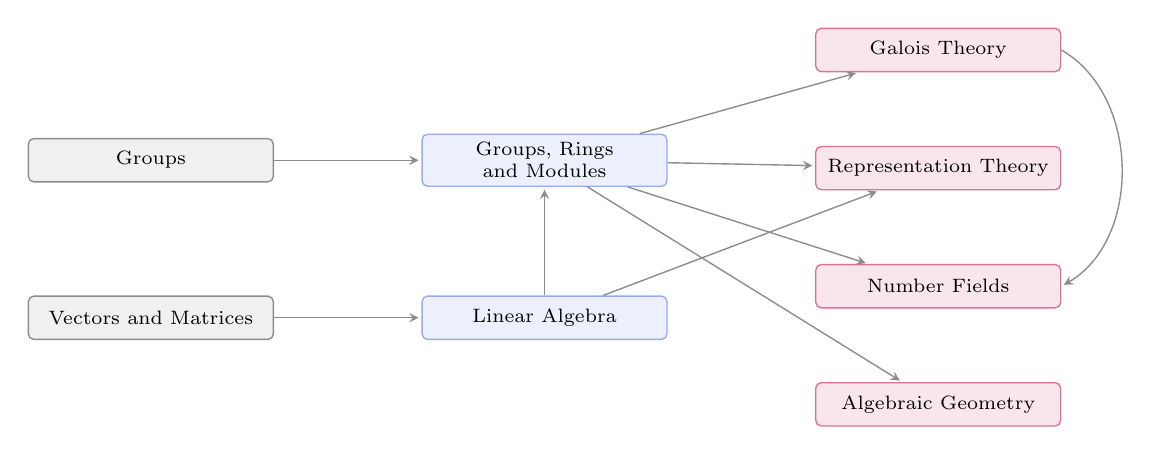
\begin{tikzpicture}
	\node[depia] (grp)  at (0,1.0)    {Groups};
	\node[depia] (vm)   at (0,-1.0)   {Vectors and Matrices};
	\node[depib] (grm)  at (5,1.0)    {Groups, Rings and Modules};
	\node[depib] (la)   at (5,-1.0)   {Linear Algebra};
	\node[depii] (gal)  at (10,2.4)   {Galois Theory};
	\node[depii] (rep)  at (10,0.9)   {Representation Theory};
	\node[depii] (nf)   at (10,-0.6)  {Number Fields};
	\node[depii] (ag)   at (10,-2.1)  {Algebraic Geometry};
	\draw[deparrow] (grp) -- (grm);
	\draw[deparrow] (vm)  -- (la);
	\draw[deparrow] (la)  -- (grm);
	\draw[deparrow] (grm) -- (gal);
	\draw[deparrow] (grm) -- (rep);
	\draw[deparrow] (grm) -- (nf);
	\draw[deparrow] (grm) -- (ag);
	\draw[deparrow] (la)  -- (rep);
	\draw[deparrow] (gal.east) to[bend left=60] (nf.east);
\end{tikzpicture}
\end{center}

\subsection*{Analysis}

Everything here descends from the $\epsilon$--$N$ definition of a limit in Analysis I\@.
Analysis and Topology is the pivot: it replaces $\R$ by a metric or topological space,
and once that is done the three Part II analysis courses become possible. Analysis of
Functions also assumes the measure theory built in Probability and Measure, and repays
the Hahn--Banach and Baire theorems of Linear Analysis.

\begin{center}
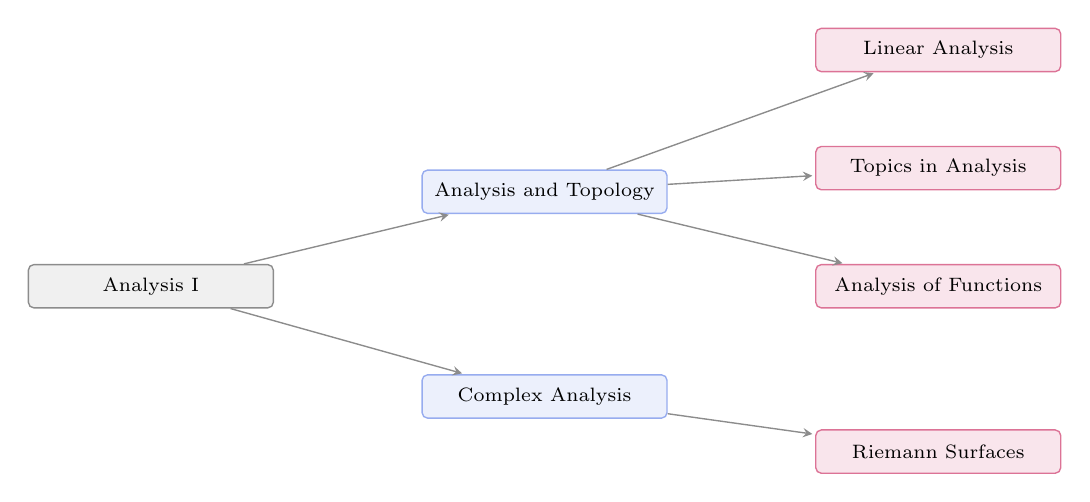
\begin{tikzpicture}
	\node[depia] (an1) at (0,0)      {Analysis I};
	\node[depib] (at)  at (5,1.2)    {Analysis and Topology};
	\node[depib] (ca)  at (5,-1.4)   {Complex Analysis};
	\node[depii] (lin) at (10,3.0)   {Linear Analysis};
	\node[depii] (tia) at (10,1.5)   {Topics in Analysis};
	\node[depii] (aof) at (10,0.0)   {Analysis of Functions};
	\node[depii] (rs)  at (10,-2.1)  {Riemann Surfaces};
	\draw[deparrow] (an1) -- (at);
	\draw[deparrow] (an1) -- (ca);
	\draw[deparrow] (at)  -- (lin);
	\draw[deparrow] (at)  -- (tia);
	\draw[deparrow] (at)  -- (aof);
	\draw[deparrow] (ca)  -- (rs);
\end{tikzpicture}
\end{center}

\subsection*{Geometry and topology}

Two strands that meet in Part II\@. One is metric and computational, running from the
curves and surfaces of Vector Calculus through Geometry to Differential Geometry; the
other is the topology introduced in Analysis and Topology, which Algebraic Topology
turns into a machine for telling spaces apart. Riemann Surfaces sits at the junction,
needing complex analysis for its local theory and covering spaces for its global one.

\begin{center}
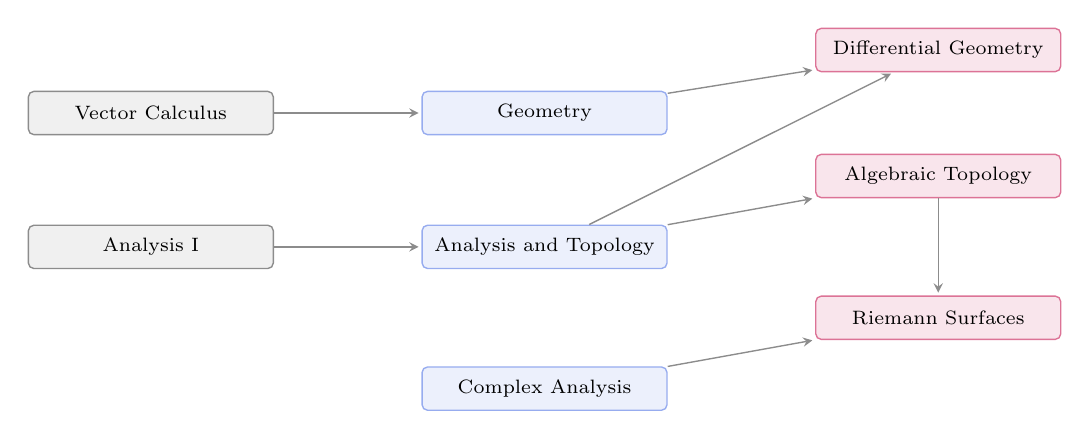
\begin{tikzpicture}
	\node[depia] (vc)  at (0,0.8)    {Vector Calculus};
	\node[depia] (an1) at (0,-0.9)   {Analysis I};
	\node[depib] (geo) at (5,0.8)    {Geometry};
	\node[depib] (at)  at (5,-0.9)   {Analysis and Topology};
	\node[depib] (ca)  at (5,-2.7)   {Complex Analysis};
	\node[depii] (dg)  at (10,1.6)   {Differential Geometry};
	\node[depii] (alt) at (10,0.0)   {Algebraic Topology};
	\node[depii] (rs)  at (10,-1.8)  {Riemann Surfaces};
	\draw[deparrow] (vc)  -- (geo);
	\draw[deparrow] (an1) -- (at);
	\draw[deparrow] (geo) -- (dg);
	\draw[deparrow] (at)  -- (alt);
	\draw[deparrow] (at)  -- (dg);
	\draw[deparrow] (alt) -- (rs);
	\draw[deparrow] (ca)  -- (rs);
\end{tikzpicture}
\end{center}

\subsection*{Probability and statistics}

Part IA Probability is combinatorial and concrete; Probability and Measure goes back
and rebuilds it on the measure theory of Analysis and Topology, at which point the
limit theorems become theorems rather than slogans. Stochastic Financial Models is
where the whole strand, optimisation included, is put to work.

\begin{center}
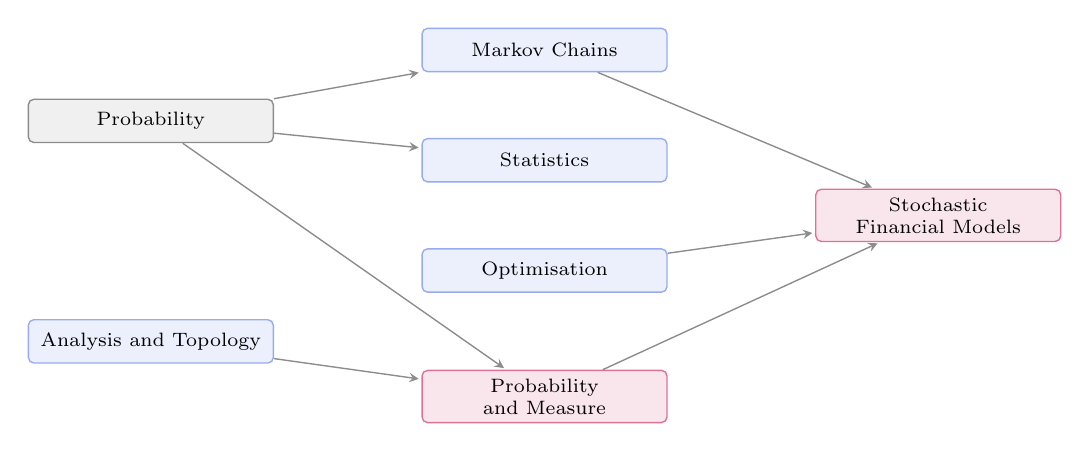
\begin{tikzpicture}
	\node[depia] (pr)  at (0,1.0)    {Probability};
	\node[depib] (at)  at (0,-1.8)   {Analysis and Topology};
	\node[depib] (mc)  at (5,1.9)    {Markov Chains};
	\node[depib] (st)  at (5,0.5)    {Statistics};
	\node[depib] (opt) at (5,-0.9)   {Optimisation};
	\node[depii] (pm)  at (5,-2.5)   {Probability and Measure};
	\node[depii] (sfm) at (10,-0.2)  {Stochastic\\Financial Models};
	\draw[deparrow] (pr)  -- (mc);
	\draw[deparrow] (pr)  -- (st);
	\draw[deparrow] (pr)  -- (pm);
	\draw[deparrow] (at)  -- (pm);
	\draw[deparrow] (mc)  -- (sfm);
	\draw[deparrow] (opt) -- (sfm);
	\draw[deparrow] (pm)  -- (sfm);
\end{tikzpicture}
\end{center}

\subsection*{Methods and mathematical physics}

The applied side of the book. Differential Equations and Vector Calculus supply the
machinery, Dynamics and Relativity supplies the physics, and the Part IB courses are
where the two are finally allowed to meet. Note how much converges on Methods: Fourier
series, Sturm--Liouville theory and Green's functions are the common language of almost
everything applied that follows, and it is Methods that supplies Quantum Mechanics with
the separation of variables and the special functions it needs in three dimensions.

\begin{center}
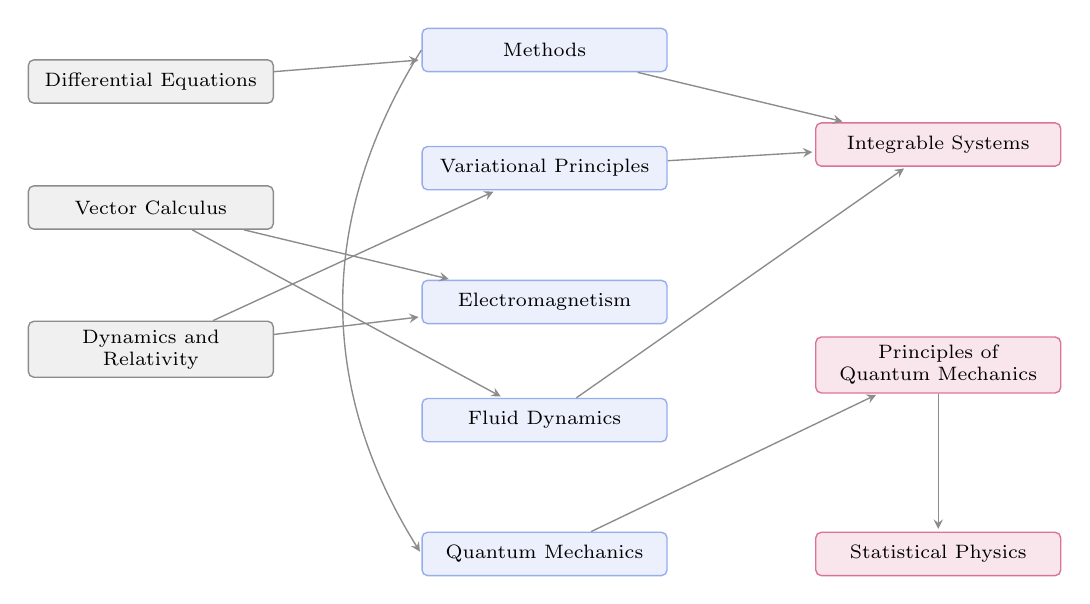
\begin{tikzpicture}
	\node[depia] (de)  at (0,2.0)    {Differential Equations};
	\node[depia] (vc)  at (0,0.4)    {Vector Calculus};
	\node[depia] (dr)  at (0,-1.4)   {Dynamics and Relativity};
	\node[depib] (me)  at (5,2.4)    {Methods};
	\node[depib] (vp)  at (5,0.9)    {Variational Principles};
	\node[depib] (em)  at (5,-0.8)   {Electromagnetism};
	\node[depib] (fd)  at (5,-2.3)   {Fluid Dynamics};
	\node[depib] (qm)  at (5,-4.0)   {Quantum Mechanics};
	\node[depii] (is)  at (10,1.2)   {Integrable Systems};
	\node[depii] (pqm) at (10,-1.6)  {Principles of\\Quantum Mechanics};
	\node[depii] (sp)  at (10,-4.0)  {Statistical Physics};
	\draw[deparrow] (de) -- (me);
	\draw[deparrow] (me.west) to[bend right=32] (qm.west);
	\draw[deparrow] (vc) -- (em);
	\draw[deparrow] (vc) -- (fd);
	\draw[deparrow] (dr) -- (vp);
	\draw[deparrow] (dr) -- (em);
	\draw[deparrow] (me) -- (is);
	\draw[deparrow] (vp) -- (is);
	\draw[deparrow] (fd) -- (is);
	\draw[deparrow] (qm) -- (pqm);
	\draw[deparrow] (pqm) -- (sp);
\end{tikzpicture}
\end{center}

\subsection*{Discrete mathematics, logic and computation}

The most self-contained group in the book, and the natural place to start if you want
to read a Part II course without first reading two years of anything. Numbers and Sets
is very nearly the only prerequisite, and most of what it supplies is the habit of
proof rather than any particular theorem.

\begin{center}
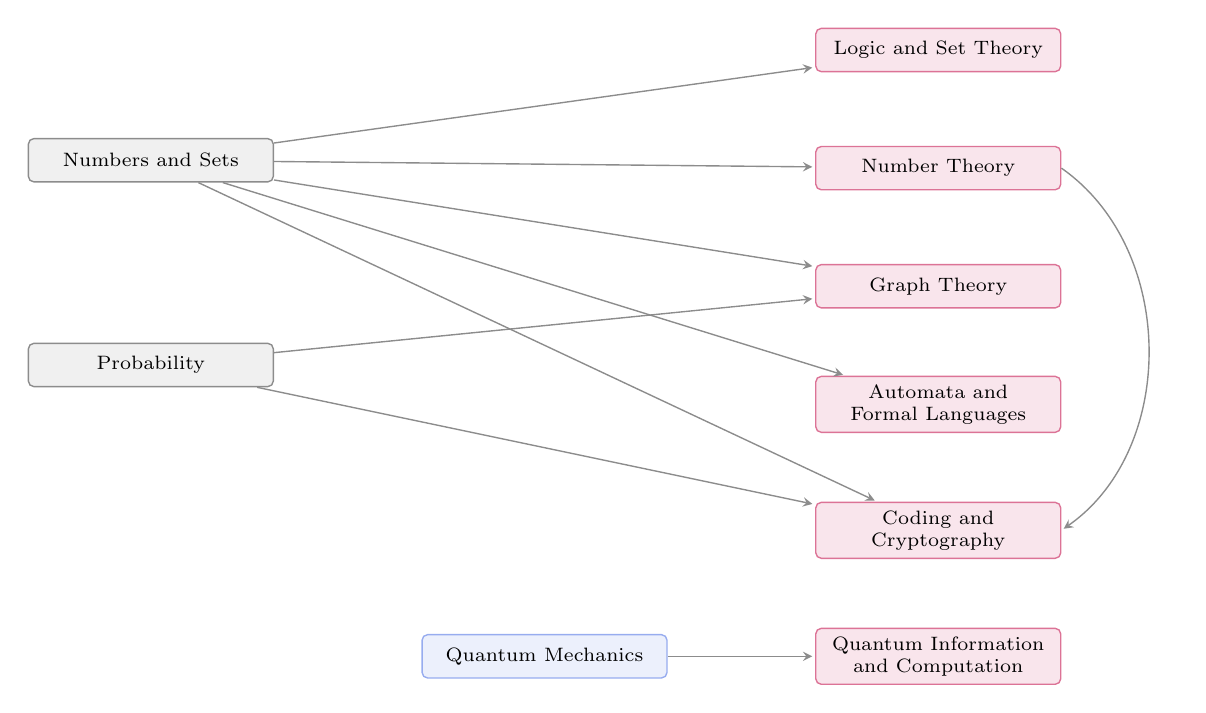
\begin{tikzpicture}
	\node[depia] (ns)  at (0,1.6)    {Numbers and Sets};
	\node[depia] (pr)  at (0,-1.0)   {Probability};
	\node[depib] (qm)  at (5,-4.7)   {Quantum Mechanics};
	\node[depii] (lst) at (10,3.0)   {Logic and Set Theory};
	\node[depii] (nt)  at (10,1.5)   {Number Theory};
	\node[depii] (gt)  at (10,0.0)   {Graph Theory};
	\node[depii] (afl) at (10,-1.5)  {Automata and Formal Languages};
	\node[depii] (cc)  at (10,-3.1)  {Coding and Cryptography};
	\node[depii] (qic) at (10,-4.7)  {Quantum Information and Computation};
	\draw[deparrow] (ns) -- (lst);
	\draw[deparrow] (ns) -- (nt);
	\draw[deparrow] (ns) -- (gt);
	\draw[deparrow] (ns) -- (afl);
	\draw[deparrow] (ns) -- (cc);
	\draw[deparrow] (pr) -- (gt);
	\draw[deparrow] (pr) -- (cc);
	\draw[deparrow] (qm) -- (qic);
	\draw[deparrow] (nt.east) to[bend left=55] (cc.east);
\end{tikzpicture}
\end{center}

\section*{The colours}

The notes lean fairly heavily on coloured panels, and once you know the scheme you can
navigate a chapter by scanning it. Everything in a coloured box is a formal statement;
everything between the boxes is me talking.

\begin{itemize}
	\item \textcolor{definitionfg}{\textbf{Pale green, with a teal heading}} is a
	\emph{definition}. Axioms and physical laws share this colour, on the grounds that
	they too are things being stipulated rather than deduced.

	\item \textcolor{theoremfg}{\textbf{Pale lilac, with a dark blue heading}} is a
	\emph{result}: theorems, propositions, lemmas, corollaries, facts and claims all
	live here. There is no significance to the choice between those words beyond the
	usual one of importance.

	\item \textcolor{examplefg}{\textbf{Pale pink, with a rust-coloured heading}} is an
	\emph{example} or a question. These are usually worked, and they are usually the
	fastest way into a section you find opaque.

	\item \textbf{Grey, with a rule down the left-hand edge}, is a \emph{proof}. The rule
	runs the height of the argument, so you can see at a glance where a long proof ends
	and the discussion starts again.

	\item \textcolor{blue}{\textbf{Bold blue}} in running text marks a term at the point
	where it is defined.
\end{itemize}

A word of warning about the pale green boxes in particular. Because definitions are so
visually distinctive it is tempting to read only those, which is exactly the wrong way
round: the prose between the boxes is where any motivation lives, and in these notes
there is not so much of it that you can afford to skip it.

\section*{A closing caution}

These are lecture notes, and they behave like lecture notes. Sometimes a chapter
develops an idea patiently over three pages; sometimes it disposes of an entire lecture
in half a column because that was all the reminder I needed. If you hit a passage that
seems to assume you already understand it, that is usually because it was written by
somebody who had just been told it, for somebody who was about to be examined on it.
Read around it, come back, and it generally opens up.
